Sicherheitsrisiken in virtualisierten Netzinfrastrukturen lassen sich auf verschiedene Weisen wie z.B. nach ISO/OSI-Schicht, nach Verletzung der klassischen C.I.A.-Aspekte, [nach Schicht in der NV-Architektur,] oder aus Sicht des SPs bzw. InPs klassifizieren. Da dieses Kapitel sich aber auf durch Netzvirtualisierung gegenüber herkömmlichen Netzinfrastrukturen neu hinzukommende Risiken konzentriert, liegt der folgenden Klassifizierung zur Verdeutlichung der Angriffswege die in Abbildung \ref{fig:gefahren_klassifizierung} dargestellte Struktur zugrunde, die sich auf der Drei-Schichtenarchitektur virtualisierter Netze (Abbildung \ref{fig:gefahren_dreiEbenenDerVirtualisierung}) ableitet.

Sicherheitsrisiken werden zunächst nach solchen technischer, organisatorischer bzw. unternehmerischer und rechtlicher Art geordnet. Im Zentrum der Betrachtung stehen dabei die technischen Risiken, welche wiederum nach Angriffsrichtungen ‚\textit{von NI ausgehend}‘, ‚\textit{vom VN ausgehend}‘ und ‚\textit{vom User ausgehend}‘ gegliedert werden sollen. In jeder dieser Kategorien wird nach Angriffsziel ‚\textit{gegen NI}‘, ‚\textit{gegen VN/VM}‘ und ‚\textit{gegen User}‘ unterteilt. \\
Da die Kategorien ‚\textit{von NI ausgehend gegen NI}‘, ‚\textit{von VN ausgehend gegen User}‘[AUCH DAS?] und ‚\textit{vom User ausgehend gegen User}‘ in virtualisierten Netzwerkumgebungen keine neuen Angriffsszenarien zu eröffnen scheinen, werden sie hier dem Ziel des Kapitels entsprechend nicht tiefergehend ausgeführt. 


\begin{figure}[htb]
	\begin{center}
	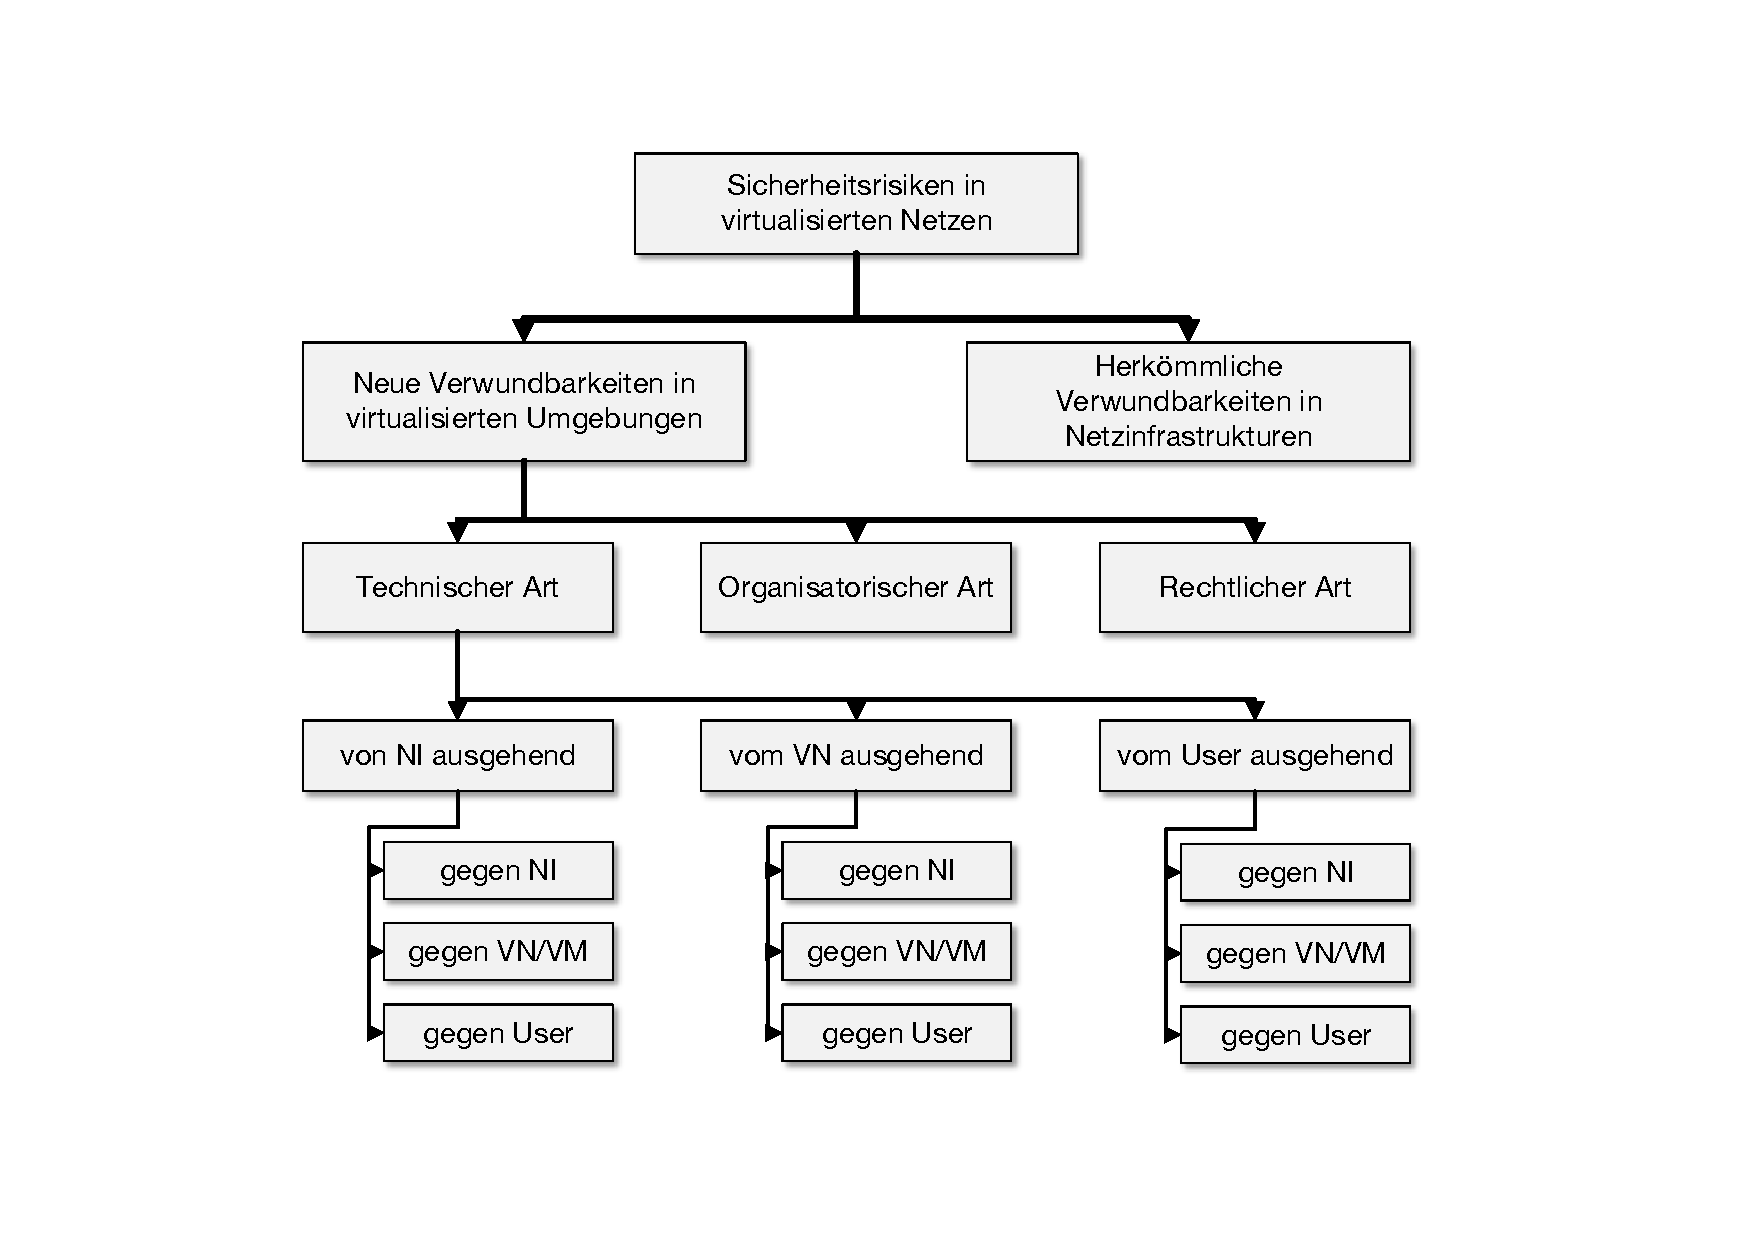
\includegraphics[width=\textwidth]{gefahren_klassifizierung.pdf}
	\caption{\label{fig:gefahren_klassifizierung} Klassifizierung von Gefahren in virtualisierten Netzwerken. 
		\newline NI = Netzwerkinfrastruktur / Substratnetz. Der physische Host einer VM ist Teil der NI.
		\newline User = Endsystem bzw. in VNs implementierter Service oder Nutzer.}
	\end{center}
\end{figure}





\subsubsection{Technischer Art}
\label{subsubsec:gefahren_virt_technisch}
[KURZE EINLEITUNG?]


\paragraph{Von NI ausgehend gegen VN und User.}
\label{parag:vonNI}
Physische Hosts bieten ihren VMs Ressourcen an. Alle Dienste und Anwendungen der VMs werden letztlich auf dem physischen Host ausgeführt und auch alle Daten auf ihm gespeichert. Dies eröffnet für den physischen Host prinzipiell die Möglichkeit eines Monitorings der VM-Aktivitäten, was ab einer gewissen Intensität sicherlich über Verwaltungsbelange hinausgehen und Privatsphärenanforderungen widersprechen dürfte. Auf demselben Weg lassen sich auch vertraulichkeitsverletzende Sniffing- oder Spoofing-Attacken gegen VM bzw. VN starten. \\
Da alle ihre Rechenoperationen letztlich auf dem physischen Host ausgeführt werden, ist es für eine VM nur schwer möglich sich gegen solche Angriffe zu wehren. [VERSCHLÜSSELUNG ALS AUSWEG?]\\
Auch Manipulation des legitimen Datenverkehrs, (gezieltes) Verwerfen von empfangenen Paketen bzw. das Einschleusen schadhafter Nachrichten bieten eine weitere Möglichkeit der Kompromittierung, gegen die VNs und Endsysteme wohl schutzlos ausgeliefert ist.
[AUSFÜHRLICHER?]\\
Durch derartige Aktionen oder auch unzureichende Sicherungsmaßnahmen gegen Datenabfluss kann der physische Host in den SLAs vereinbarte Bestimmungen verletzen, was gerade bei Drittanbietern als Hostingpartner eine Rolle spielt.
%%%%% Angriffe von Komponenten der NI untereinander werden hier nicht beachtet.[Bereits weiter oben gesagt.]



\paragraph{Von VN/VM ausgehend}
\label{parag:vonVN}
[MINI EINLEITUNG]

\begin{itemize}
\item \textbf{Von VM/VM ausgehend gegen NI/ihren physischen Host.~~}
Das Bereitstellen von Ressourcen für VMs ist aber auch für den physischen Host nicht ohne Risiko. Schadhafte oder bösartige VMs können Verwundbarkeiten ihres physischen Host über zugeteilte Ressourcen angreifen. Ohne hinreichende Restriktionen könnte eine VM dann über ihr zugeteiltes Kontingent hinaus bspw. wichtige Speicherbereiche manipulieren oder durch übermäßige Reservierung von CPU-Zeiten eine Denail of Service Attacke gegen den physischen Host bzw. das Substratnetz fahren. Da Host und virtuelle Netztopologie aus der Ferne konfigurierbar sind, stellt das Einschleusen von konstruierten Nachrichten des verwendeten Netzwerkmanagementprotokolls auf oder durch die Netzwerkkarte des physischen Hosts einen weiteren gefährlichen Angriffsvektor dar.\\
Nach Eindringen in oder Übernahme des Hosts, einem „break of isolation“ im ersten Sinne \cite{wu2010network}, könnte eine schadhafte VM dann ihr Kontingent an Ressourcen beeinflussen, netztopologische Informationen sammeln, andere Netzwerkressourcen oder -infrastrukturkomponenten angreifen und so beispielsweise Dienste anderer VMs oder VNs behindern.

\item \textbf{Von VM/VN ausgehend gegen VM/VN.~~}
Neben den herkömmlichen Angriffsszenarien zwischen Maschinen im selben Netzwerk, ergeben sich v. a. aus der gemeinsamen Nutzung von Ressourcen neue Angriffsvektoren. 
\footnote{Da die Angriffstechniken von VMs gegen VMs auf anderen physischen Hosts vergleichbar mit herkömmlichen Angriffen in nicht-virtualisierten Netzinfrastrukturen sein dürfte, werden hier hauptsächlich VMs auf demselben physischen Host betrachtet.} 
Ein Angreifer kann sich nun gezielt Ressourcen auf denjenigen physischen Maschinen mieten, von denen auch sein Angriffsziel gehostet wird, um so erleichterten Zugang zu deren Verwundbarkeiten zu erlangen. Durch Eindringen oder Übernehmen gewisser Ressourcen des gemeinsamen physischen Hosts kann eine schadhafte VM dann ggfs. Verwundbarkeiten ausnutzen oder durch Cross-VN-side-channel-Attacken vertrauliche Informationen gewinnen und Daten manipulieren. Ein Beispiel einer Integritätsverletzung mittels einer solchen Attacke findet sich in \cite{ristenpart2009hey}. \\
Da i.d.R. [ANGABE?] werden nur virtuelle Netzwerkkarten zugeteilt, kann jede VM potentiell den gesamten Datenverkehr aller VMs bzw. VNs auf derselben physischen Netzwerkkarte lesen. Ein Monitoring anderer VMs auch aus anderen VNs, ein „break of Isolation“ im zweiten Sinne bedroht deren Vertraulichkeit. Durch Belauschen des Netzwerkverkehrs lassen sich ggfs. auch Dienste gemeinsam gehosteter VN reproduzieren und dadurch bspw. ein live Videostreaming breiter zugänglich machen.\cite{natarajansecurity}\\
Sollte es einer VM gelingen kritische Teile ihres physischen Hosts zu übernehmen, so stehen ihr zusätzlich die im Abschnitt \textit{\nameref{parag:vonNI}} aufgeführten Angriffsvektoren offen.


\item \textbf{Von VM ausgehend gegen User.~~}
Auch ein virtuelles Netzwerk kann mit herkömmlichen Methoden wie Monitoring der Nuteraktivitäten oder dem Einschleusen von konstruierten Nachrichten zur Störung oder Abbruch von Peer-to-Peer-Verbindungen Einfluss auf den Nutzverkehr seiner User nehmen.
\end{itemize}



\paragraph{Vom User ausgehend}
\label{parag:vonUser}
Einem Benutzer oder schadhaften Anwendungsprogramm stehen auch in virtualisierten Netzwerkumgebungen die bekannten Methoden der Störung durch z.B. Herbeiführen von Überlastsituationen in NV oder NI offen.

\begin{itemize}
	\item \textbf{Vom User ausgehend gegen NI.~~}
	Da sich die virtuelle Netztopologie im VNE laufend ändert, müssen Netzwerkkomponenten wie Switches und Router dynamisch umprogrammierbar sein. Dies ermächtigt Angreifer aber solche ggfs. mit Codeexpliots wie Bufferoverflows o. Ä. zu kompromittieren und für ihre Zwecke zu nutzen oder einen Denail of Service herbeizuführen.\\
	Daneben besteht die Chance auch Netzwerkknoten anzugreifen. Gelingt es z.B. mit einem Rootkit wie BluePill \cite{rutkowska2008bluepilling} (als Vorbereitung für weitere Angriffe) einen Hypervisor zu übernehmen, wird so gleichzeitig die Kontrolle über alle gehosteten VMs erlangt. Auch eine VM lässt sich als Rootkit instrumentalisieren.\cite{wu2010network}
	\item \textbf{Vom User ausgehend gegen VN.~~}
	Aus der dynamischen Natur virtueller Netzwerktopologien ergeben sich neue Verwundbarkeiten: Während der Migration im Livebetrieb eines VNs ist eine Man-in-the-Middle-Attacke möglich, mit der Informationen über und Inhalte des migrierenden VNs erlangt werden können. \cite{natarajansecurity} Auch die Manipulation von Speicherbereichen der VMs ist während der Migration möglich und lässt sich sogar automatisieren.\cite{oberheide2008empirical}\\
	Die Notwendigkeit die gesamte virtuelle Netzwerkstruktur aus der Ferne umkonfigurieren zu können, erschließt weitere Angriffsziele: Attacken auf die VN-Managementtools durch z.B. Cross-Site-Scripting, SQL-Injection etc. werden lohnend, da auf diese Weise effizient Kontrolle über das gesamte Netzwerk gewonnen werden kann.	
	\item \textbf{Vom User gegen User.~~}
	[ALLES "HERKÖMMLICH"?]
\end{itemize}

[TABELLE DER RISIKEN?]



[UNTERKAPITELZUSAMMENFASSUNG]


\subsubsection{Organisatorischer Art}
\label{subsubsec:gefahren_virt_organisatorisch}
[TODO / AUSFORMULIEREN]

Unter ‚organisatorischen‘ Risiken werden hier Risiken für Unternehmen oder im menschlichen Umgang betrachtet, die im Zusammenhang mit Virtualisierung stehen.

Wie im Kapitel \nameref{subsubsec:gefahren_virt_technisch} dargestellt, eröffnet Netzvirtualisierung eine Reihe neuer Verwundbarkeiten für gehostete Systeme. Gerade für Unternehmen dürfte die teils deutliche Gefährdung der Vertraulichkeit und Integrität von Firmen- oder Kundendaten ein ernstzunehmendes Problem darstellen. Da Netzvirtualisierung oftmals via Cloudcomputing abgewickelt wird, erhöht sich das Risiko eines Datenlecks nochmals durch den Up- und Downloadprozess von Daten.

Substratnetzprovider ist auch ein Unternehmen/Dienstleister, der sich organisatorisch verändert oder z.B. Insolvenz anmelden kann.

Snapshot-Problem. Momentanaufnahme der virt. Maschine für Backup- oder Migrationszwecke. 
\begin{itemize}
\item Einfachheit dessen ist großer Vorteil von VMs. 
\item Nachteil: Nach dem Wiedereinspielen werden ggfs. zwischenzeitlich deaktivierte Accounts oder veraltete Sicherheitsrichtlinien wieder produktiv gesetzt.
\item Virtuelle Maschinen entstehen schnell. Probleme bei Patchmanagement 
\item VMs zeitweise/Häufig deaktiviert/offline
\begin{itemize}
	\item Erhalten keine Patches am Patchday.
	\item Würmer infizieren meist relativ schnell alle verwundbaren Systeme. Geht die VM danach offline wird Malware darin nicht entfernt und die Wurminfektionwelle startet beim erneuten Onlinegehen der VM.
\end{itemize}
\item Rücksetzen/rollback einer VM kann zwischenzeitlich gepatchte Schwachstellen wieder offenbaren (Snapshot-Problem)
\end{itemize}





\subsubsection{Rechtlicher Art}
\label{subsubsec:gefahren_virt_rechtlich}
[TODO]
Da Substratnetze nicht zwingend räumlich eng beschränkt sein müssen, könnte es passieren, dass gewisse Teile des virtuellen Netzes dynamisch auf Knoten in einem anderen Land abgebildet werden, welches mit den Auflagen des Unternehmens zu Datenschutz, Privatsphäre oder IT-Securitystandards nicht vereinbar ist. \\
Aus technischen Gefahren resultierende Risiken (Sniffing vs. Datenschutz, Leaks, …)